% Opcje klasy 'iithesis' opisane sa w komentarzach w pliku klasy. Za ich pomoca
% ustawia sie przede wszystkim jezyk i rodzaj (lic/inz/mgr) pracy, oraz czy na
% drugiej stronie pracy ma byc skladany wzor oswiadczenia o autorskim wykonaniu.
\documentclass[declaration,shortabstract]{iithesis}

\usepackage[utf8]{inputenc}

%%%%% DANE DO STRONY TYTUŁOWEJ
% Niezaleznie od jezyka pracy wybranego w opcjach klasy, tytul i streszczenie
% pracy nalezy podac zarowno w jezyku polskim, jak i angielskim.
% Pamietaj o madrym (zgodnym z logicznym rozbiorem zdania oraz estetyka) recznym
% zlamaniu wierszy w temacie pracy, zwlaszcza tego w jezyku pracy. Uzyj do tego
% polecenia \fmlinebreak.
\polishtitle    {Zastosowanie technologii React i Ruby on Rails w tworzeniu aplikacji webowych na przykładzie serwisu blogowego}
\englishtitle   {Application React and Ruby on Rails to create web applications by the example of blog site}

\polishabstract {Celem pracy było opracowanie oraz implementacja platformy blogowej łączącej funkcje popularnych serwisów. Do realizacji projektu użyto nowoczesnych rozwiązań. System składa się z dwóch części. Aplikacji serwerowej napisanej w języku Ruby z wykorzystaniem Ruby on Rails oraz strony internetowej będącej interfejsem użytkownika zaimplementowanej za pomocą popularnego frameworka React }

\englishabstract{The purpose of the study was to develop the blog platform that combines the functionality of popular services. Modern solutions were used to implement this project. The system comprises of two parts. Server application was written in Ruby using Ruby on Rails and website that is a user interface was implemented using popular framework React.}
% w pracach wielu autorow nazwiska mozna oddzielic poleceniem \and
\author         {}
% w przypadku kilku promotorow, lub koniecznosci podania ich afiliacji, linie
% w ponizszym poleceniu mozna zlamac poleceniem \fmlinebreak
\advisor        {}
\date          {}                     % Data zlozenia pracy
% Dane do oswiadczenia o autorskim wykonaniu
\transcriptnum {}                     % Numer indeksu
\advisorgen    {} % Nazwisko promotora w dopelniaczu
%%%%%
\usepackage{graphicx, xcolor}
%%%%% WLASNE DODATKOWE PAKIETY
%
%\usepackage{graphicx,listings,amsmath,amssymb,amsthm,amsfonts,tikz}
%
%%%%% WŁASNE DEFINICJE I POLECENIA
%
%\theoremstyle{definition} \newtheorem{definition}{Definition}[chapter]
%\theoremstyle{remark} \newtheorem{remark}[definition]{Observation}
%\theoremstyle{plain} \newtheorem{theorem}[definition]{Theorem}
%\theoremstyle{plain} \newtheorem{lemma}[definition]{Lemma}
%\renewcommand \qedsymbol {\ensuremath{\square}}
% ...
%%%%%

\begin{document}

%%%%% POCZĄTEK ZASADNICZEGO TEKSTU PRACY

\chapter{Wprowadzenie}
Tematem pracy jest aplikacja internetowa implementująca wybrane funkcje platformy blogowej. Dzisiaj internet jest przepełniony treściami tworzonymi przez jego użytkowników np. za pomocą wpisów na portalach społecznościowych lub artykułach na blogach. Jest to atrakcyjna przestrzeń do tworzenia nowych aplikacji pomagających dzielić się treściami. Mimo dużej konkurencji na rynku nadal istnieje zapotrzebowanie na nowe serwisy. Przykładem jest \textit{\textbf{Reddit}} założony w 2005 roku. Dziś jest piątą (według Alexa) najczęściej odwiedzaną stroną w Stanach Zjednoczonych, miesięcznie przyciągającą 330 milionów użytkowników. Na początku jej główną funkcjonalnością była możliwość dzielenia się linkami do stron przez użytkowników oraz głosowaniem i komentowanie ich. Z czasem wraz z rozwojem serwisu użytkownikom oddano możliwość dzielenia się nie tylko łączami do innych stron, ale też postami czy obrazkami. Dziś jest domem dla tysięcy społeczności. Innym przykładem jest powstały w 2012 roku \textit{\textbf{Medium}}. Platforma skupia zarówno profesjonalnych dziennikarzy, jak i amatorów. Jej głównym celem jest dostarczenie użytkownikom wartościowych treści w przyjemnej formie. W odróżnieniu od Reddita strona skupia się na udostępnianej treści, a nie na interakcjach pomiędzy użytkownikami. 

Celem jest stworzenie aplikacji webowej która ma łączyć możliwość tworzenia rozbudowanych postów zaczerpniętą z Medium oraz udostępniać użytkownikom miejsce do dyskusji na ich temat podobnie jak w Reddicie. Podczas wyboru zestawu narzędzi do realizacji implementacji pracy chciałem, aby zawierał on jak najwięcej nowych, wykorzystywanych na rynku komercyjnym rozwiązań. Co pozwoliłoby mi poszerzyć moje umiejętności. W wyniku tego zakres prac obejmuje aplikację \textbf{\textit{,,blogger-frontend"}} będącą interfejsem użytkownika oraz \textbf{\textit{,,blogger-backend"}} udostępniajace dane za pomocą API

\chapter{Opis i analiza zagadnienia}

Pierwsze blogi powstały w późnych latach 90-tych. Były prostymi, statycznymi stronami WWW aktualizowanymi ręcznie. Wpisy były wyświetlane użytkownikowi w odwrotnej chronologicznej kolejności. Wraz z upływem czasu i wzrostem popularności internetowych dzienników powstały dedykowane serwisy oraz oprogramowanie służące do ich prowadzenia. Pozwoliło to na prowadzenie własnego bloga przez przeciętnego użytkownika internetu. W dniu dzisiejszym najpopularniejszą odmianą są mikroblogi - strony umożliwiające użytkownikom dzielenie się krótkimi, kilku zdaniowymi przemyśleniami lub obrazkami np. Twitter, Facebook, Wykop.pl.

\section{Wymagania funkcjonalne}

\begin{itemize}
    \item Niezalogowany użytkownik może: 
    \begin{itemize}
         \item zalogować się do istniejącego konta
         \item utworzyć nowe konto
         \item przeglądać listę postów
         \item przeglądać post wraz z jego komentarzami
         \item przeglądać listę kategorii
         \item przeglądać posty w danej kategorii
    \end{itemize}
    \item Zalogowany użytkownik może:
        \begin{itemize}
            \item wylogować się
            \item pisać nowe posty
            \item pisać komentarze
            \item przeglądać listę powiadomień
        \end{itemize}
\end{itemize}

\section{Wymagania niefunkcjonalne}
\begin{itemize}
    \item Prosty interfejs użytkownika
    \item Bezpieczny system kont dla użytkowników
    \item Rozszerzalność
    \item Wykorzystanie narzędzi do statycznej analizy kodu
    \item Zastosowanie narzędzi do ciągłej integracji podczas wytwarzania kodu
    \item Działanie projektu na systemie Linux
    
\end{itemize}

% \subsection{Wnioski}-
\chapter{Część dla programisty}
\section{Architektura aplikacji}
Aplikacja jest napisana w architekturze klient-serwer, podczas jej tworzenia wykorzystano wzorzec separacji  zagadnień (z and. separation of concerns, SoC). Pozwoliło to na podzielenie serwisu na dwie części. Pierwszą jest warstwa dostępu do danych napisana w języku Ruby z wykorzystaniem Ruby on Rails. Odpowiada za przechowywanie danych w bazie danych PostgreSQL oraz ich udostępnienie za pomocą API. Drugą częścią jest warstwa prezentacji, wykorzystuje JavaScript oraz framework React w celu prezentacji danych. Taki podział pozwala na niezależny rozwój każdej z części aplikacji osobno.

\section{Uruchomienie aplikacji}

\subsection{Backend}
Wymagane oprogramowanie do uruchomienia aplikacji:
        \begin{itemize}
            \item Ruby w wersji 2.6.2
            \item Bundler w wersji 1.17
            \item Foreman w wersji 0.85.0
            \item Pozostałe zależności z pliku "Gemfile"
            \item PostgreSQL w wersji 11.3
            \item Redis w wersji 5.0.5
        \end{itemize}

\begin{enumerate}
    \item W katalogu \textbf{\textit{,,blogger-backend"}} poleceniem \textbf{\textit{,,bundle install"}} zainstalować dodatkowe biblioteki
    \item Wykonać migracje do bazy danych poleceniem \textbf{\textit{,,rails db:migrate"}}
    \item Poleceniem \textbf{\textit{,,foreman start -f Procfile.dev"}} uruchomić serwer
\end{enumerate}

\subsection{Frontend}
Wymagane oprogramowanie do uruchomienia aplikacji:
    \begin{itemize}
        \item Yarn w wersji 1.13.0
        \item Zależności znajdujące się w pliku "package.json" 
    \end{itemize}

\begin{enumerate}
    \item W folderze \textbf{\textit{,,bloger-frontend"}} poleceniem \textbf{\textit{,,yarn"}} zainstalować brakujące pakiety
    \item Poleceniem \textbf{\textit{"yarn start"}} uruchomić serwer deweloperski, jego domyślny adres \textit{localhost:3001}
\end{enumerate}

\section{Backend}
\subsection{Ruby on Rails}
Aplikacja serwerowa została napisana z wykorzystaniem frameworka Ruby on Rails. Powstał on w 2005 roku jako narzędzie do szybkiego tworzenia aplikacji webowych. Głównymi strategiami projektowymi są ,,Convention Over Configuration" oraz DRY (,,Don't repeat yourself"). Dzięki temu programista już po zainicjalizowaniu projektu otrzymuje domyślną strukturę oraz konfigurację pozwalającą ominąć żmudny proces ręcznego definiowania ustawień. W momencie powstania oferował wiele innowacyjnych funkcji takich jak: generowanie tabel w bazie danych na podstawie modeli, scaffolding oraz system migracji. Dzisiaj inspiracje Ruby on Rails możemy znaleźć w wielu innych frameworkach np. Django, Sails.js. Napędza serwisy takie jak GitHub, AribBnB, Kickstarter.

\subsection{Struktura aplikacji}
Struktura aplikacji serwerowej przedstawiona na rysunku \ref{fig:struktura_serwer1} oraz \ref{fig:struktura_serwer2} powstała w wyniku działania wbudowanego w Ruby on Rails generatora. Utworzył on minimalną konfigurację potrzebną do zaczęcia pracy. Najważniejszą częścią projektu jest katalog \textbf{\textit{,,app"}} to w nim znajdują się wszystkie komponent aplikacji. W podkatalogu \textbf{\textit{,,app/controllers"}} umieszczono kontrolery, odpowiadają one za nadanie sensu żądaniom jakie przychodzą do API oraz zadbaniu o wygenerowanie poprawnej odpowiedzi. W \textbf{\textit{,,app/services"}} znajdują się klasy serwisów, implementują one interakcje użytkownika z aplikacją. Pozwala to na wyodrębnienie logiki biznesowej z kontrolerów. Konfiguracje do serializera znajdują się w folderze \textbf{\textit{,,app/serializers"}}. Katalog \textbf{\textit{,,db"}} zawiera aktualny schemat bazy danych co pozwala na przenoszenie bazy pomiędzy komputerami oraz migrację czyli zestaw plików napisany w Ruby DSL pozwalający na zmianę schematu bazy danych bez potrzeby pisania ręcznie poleceń SQL.
\begin{figure}
    \centering
    \begin{minipage}[b]{0.4\textwidth}
        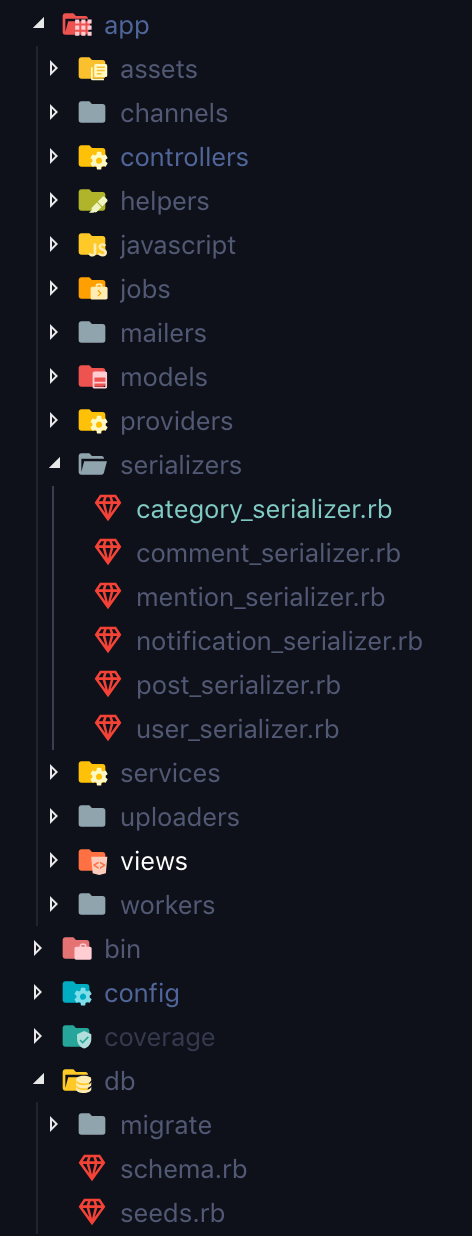
\includegraphics[width=\textwidth]{images/serwer1.png}
        \caption{Struktura aplikacji serwerowej cz. 1}
        \label{fig:struktura_serwer1}
    \end{minipage}
    \hfill
    \begin{minipage}[b]{0.4\textwidth}
        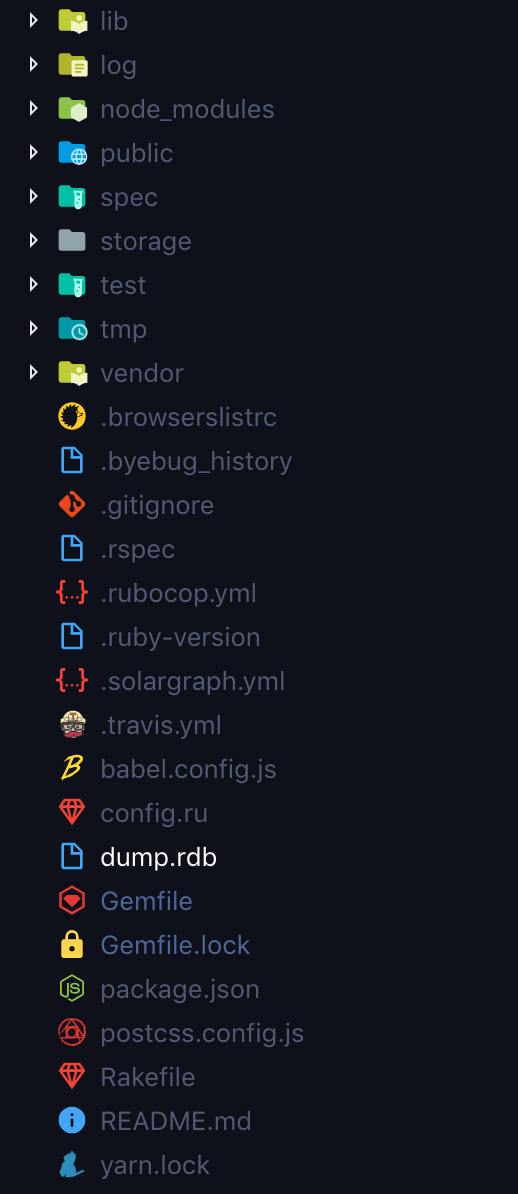
\includegraphics[width=\textwidth]{images/serwer2.png}
        \caption{Struktura aplikacji serwerowej cz.2}
        \label{fig:struktura_serwer2}
    \end{minipage}
\end{figure}

\subsection{Baza danych}
Jako system przechowywania danych wybrano PostgreSQL. Jest to otwartoźródłowy silnik do zarządzania relacyjnymi bazami danych. Charakteryzuje się on wysoką kompatybilnością ze standardem SQL:2011, zgodnością z ACID (Atomicity, Consistency, Isolation, Durability) oraz niezawodnością. Ruby on Rails w domyślnej konfiguracji zapewnia wsparcie dla Postgresa. Pozwala to na zastosowanie systemu migracji, który wraz z rozbudową aplikacji odpowiednio modyfikuje istniejący schemat bazy danych.

\subsubsection{Schemat bazy danych}
Baza danych (rys. \ref{fig:erd_diagram}) składa się z następujących tabeli: 
\begin{itemize}
    \item \textbf{users} - zawiera między innymi takie informacje jak imię, e-mail, hasło. Jest wykorzystywana podczas autentykacji.
    \item \textbf{posts} - podstawowy typ danych w platformie blogowej. Składa się z tytułu, zawartości oraz linku do miniaturki.
    \item \textbf{comments} - przechowuje zawartość komentarzy
    \item \textbf{likes} - odpowiada za przechowywania głosów użytkowników
    \item \textbf{mentions} - gromadzi dane z systemu wspomnień. Dla każdej wspomnianej osoby w komentarzu przechowuje wpis z identyfikatorem użytkownika oraz komentarzy, co pozwala na szybkie odnalezienie zarówno osób skojarzonych z wpisem, jak i postów przypisanych danej osobie.
    \item \textbf{notifications} - odpowiada za powiadomienia. Dzięki polimorficznym asocjacjom możliwa jest rozbudowa tego systemu wraz z rozwojem aplikacji. Dla każdego wpisu w tabeli pamiętane jest zarówno identyfikator powiązanego obiektu,jak i jego typ. Pozwala to, aby jedna tabela zawierała odniesienia do wielu.
\end{itemize}

\begin{figure}
    \centering
    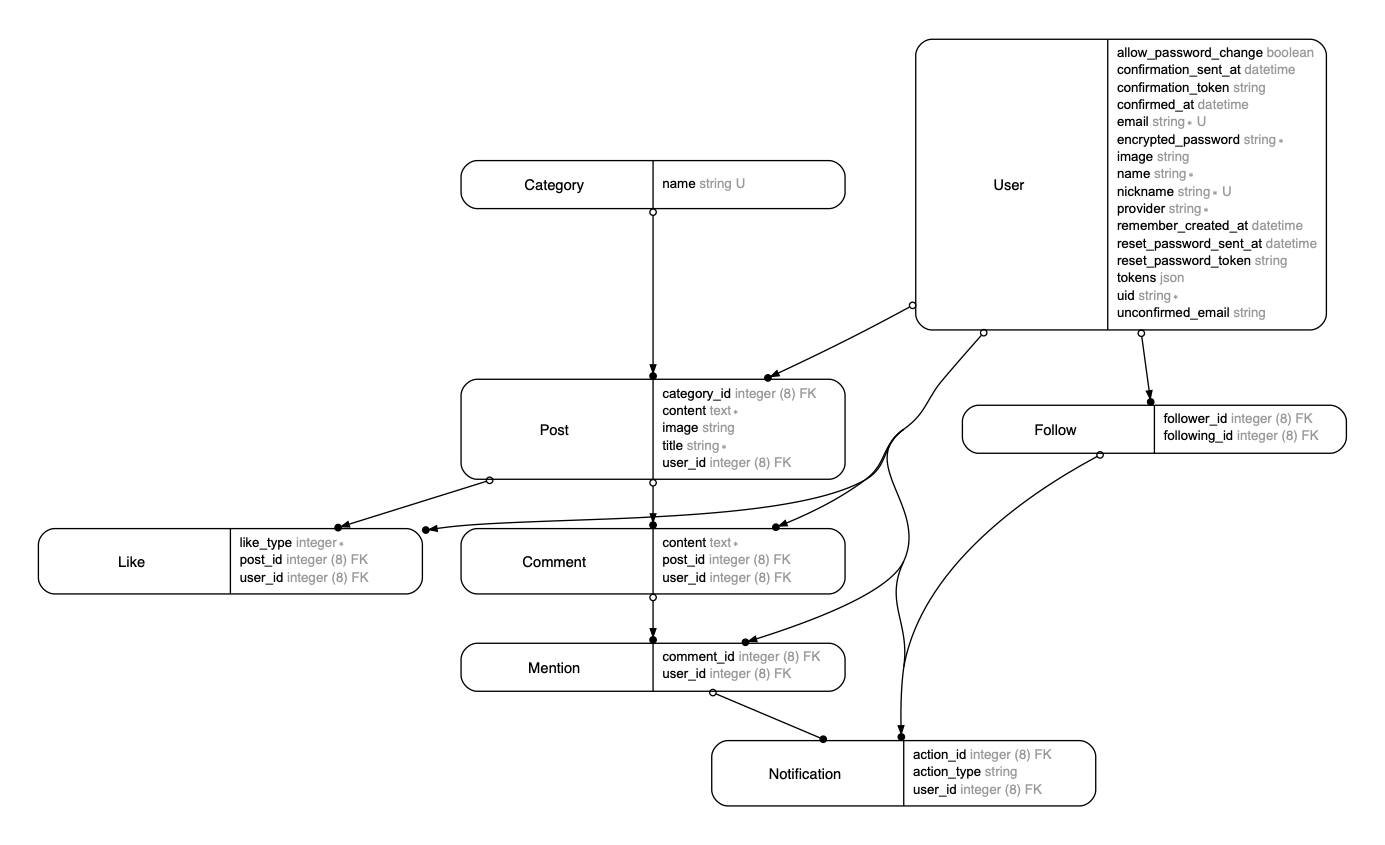
\includegraphics[width=\textwidth]{images/erd.png}
    \caption{Schemat ERD bazy danych}
    \label{fig:erd_diagram}
\end{figure}
% \subsection{Uwierzytelnianie} 
\section{Frontend}

\subsection{React}
Interfejs udostępniany użytkownikowi został napisany z wykorzystaniem Reacta. Jest to biblioteka JavaScript utworzona w 2016 roku utrzymywana przez Facebook. Dziś jest jednym z najpopularniejszych frameworków do budowy interfejsów użytkownika. Jego główną cechą charakterystyczną jest budowanie złożonych projektów za pomocą wielu mniejszych, wyizolowanych części nazywanych komponentami. Są to klasy lub funkcje, które mogą przyjmować jako wejście właściwości (\textbf{\textit{,,props"}}) a zwracają opis jak dany komponent powinien zostać wyrenderowany przez przeglądarkę. Dodatkowo React pozwala na to, aby komponenty posiadały stan, czyli zestaw danych, które może zmieniać. Biblioteka ta umożliwia również na dynamiczne modyfikowaie HTML bez potrzeby przeładowywanie strony. Istnieje możliwość wykorzystania Reacta na urządzeniach mobilnych za pomocą React Native.

\subsection{Ant Design}
W aplikacji udostępnianej klientowi bardzo ważnym elementem jest jej wygląd dlatego, aby całość aplikacji prezentowała się spójnie, zdecydowano się zastosować wytyczne Ant Design oraz ich implementację za pomocą biblioteki \textbf{\textit{,,antd"}} zawierającej zestaw komponentów React. Znacznie to zmniejszyło czas potrzebny na dodawanie stylów to nowych komponentów i pozwoliło skupić się na implementacji nowych funkcjonalności. 

\subsection{Struktura projektu}
Projekt został zainicjowany za pomocą narzędzia \textbf{\textit{,,create-react-app"}} dostarczanego przez Facebooka. Tworzy ono gotowe, skonfigurowane środowisko umożliwiające natychmiastowe rozpoczęcie pracy nad aplikacją. Kod aplikacji został podzielony w następujących folderach: 
\begin{itemize}
    \item \textbf{\textunderscore helpers} - zawiera pomocnicze funkcje nie przypisane do konkretnego komponentu.
    \item \textbf{\textunderscore services} - znajdują się tu funkcje odpowiedzialne za interakcję z API.
    \item \textbf{componets} - jest to najważniejszy folder. To w nim znajdują się wszystkie komponenty odpowiedzialne za wygląd i działanie aplikacji.
\end{itemize}
\begin{figure}
    \centering
    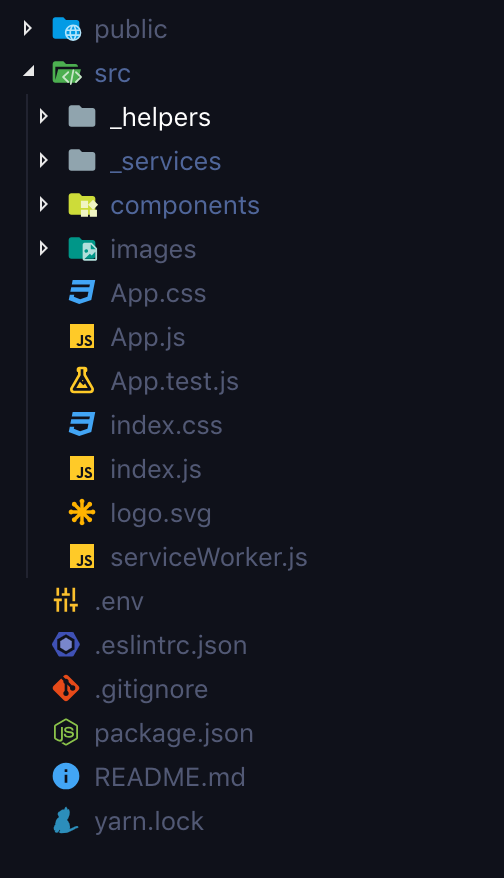
\includegraphics[]{images/forontend.png}  
    \caption{Struktura projektu}
    \label{fig:frontend_struct}
\end{figure}


\chapter{Część dla użytkownika}
\section{Opis programu}
Blogger jest platformą blogową pozwalającą użytkownika dodawać wpisy w jednej z predefiniowanych kategorii. Mogą oni również wchodzić w interakcję między sobą poprzez dyskusje pod wpisami lub system ich oceniania. Aby móc korzystać z tych funkcji wystarczy jedynie utworzyć i zweryfikować za pomocą e-mail konto.
\section{Demonstracja aplikacji}
Serwis można podzielić na dwie części, jedna dla każdego użytkownika, druga tylko dla zalogowanego.

\subsection{Niezalogowany użytkownik}
\subsubsection{Strona główna}
Użytkownik po wejściu na adres aplikacji ukaże się strona główna (rys. \ref{fig:main_page}), na której będzie mógł przeglądać listę wszystkich postów, jakie zostały utworzone. Każdy z nich jest reprezentowany przez przeglądowy opis, na który składa się: tytuł, skrócona treść wpisu oraz graficzna miniaturka. Użytkownik może zostać przeniesiony do szczegółowego widoku wpisu po kliknięciu w jeden z nich.
\begin{figure}
    \centering
    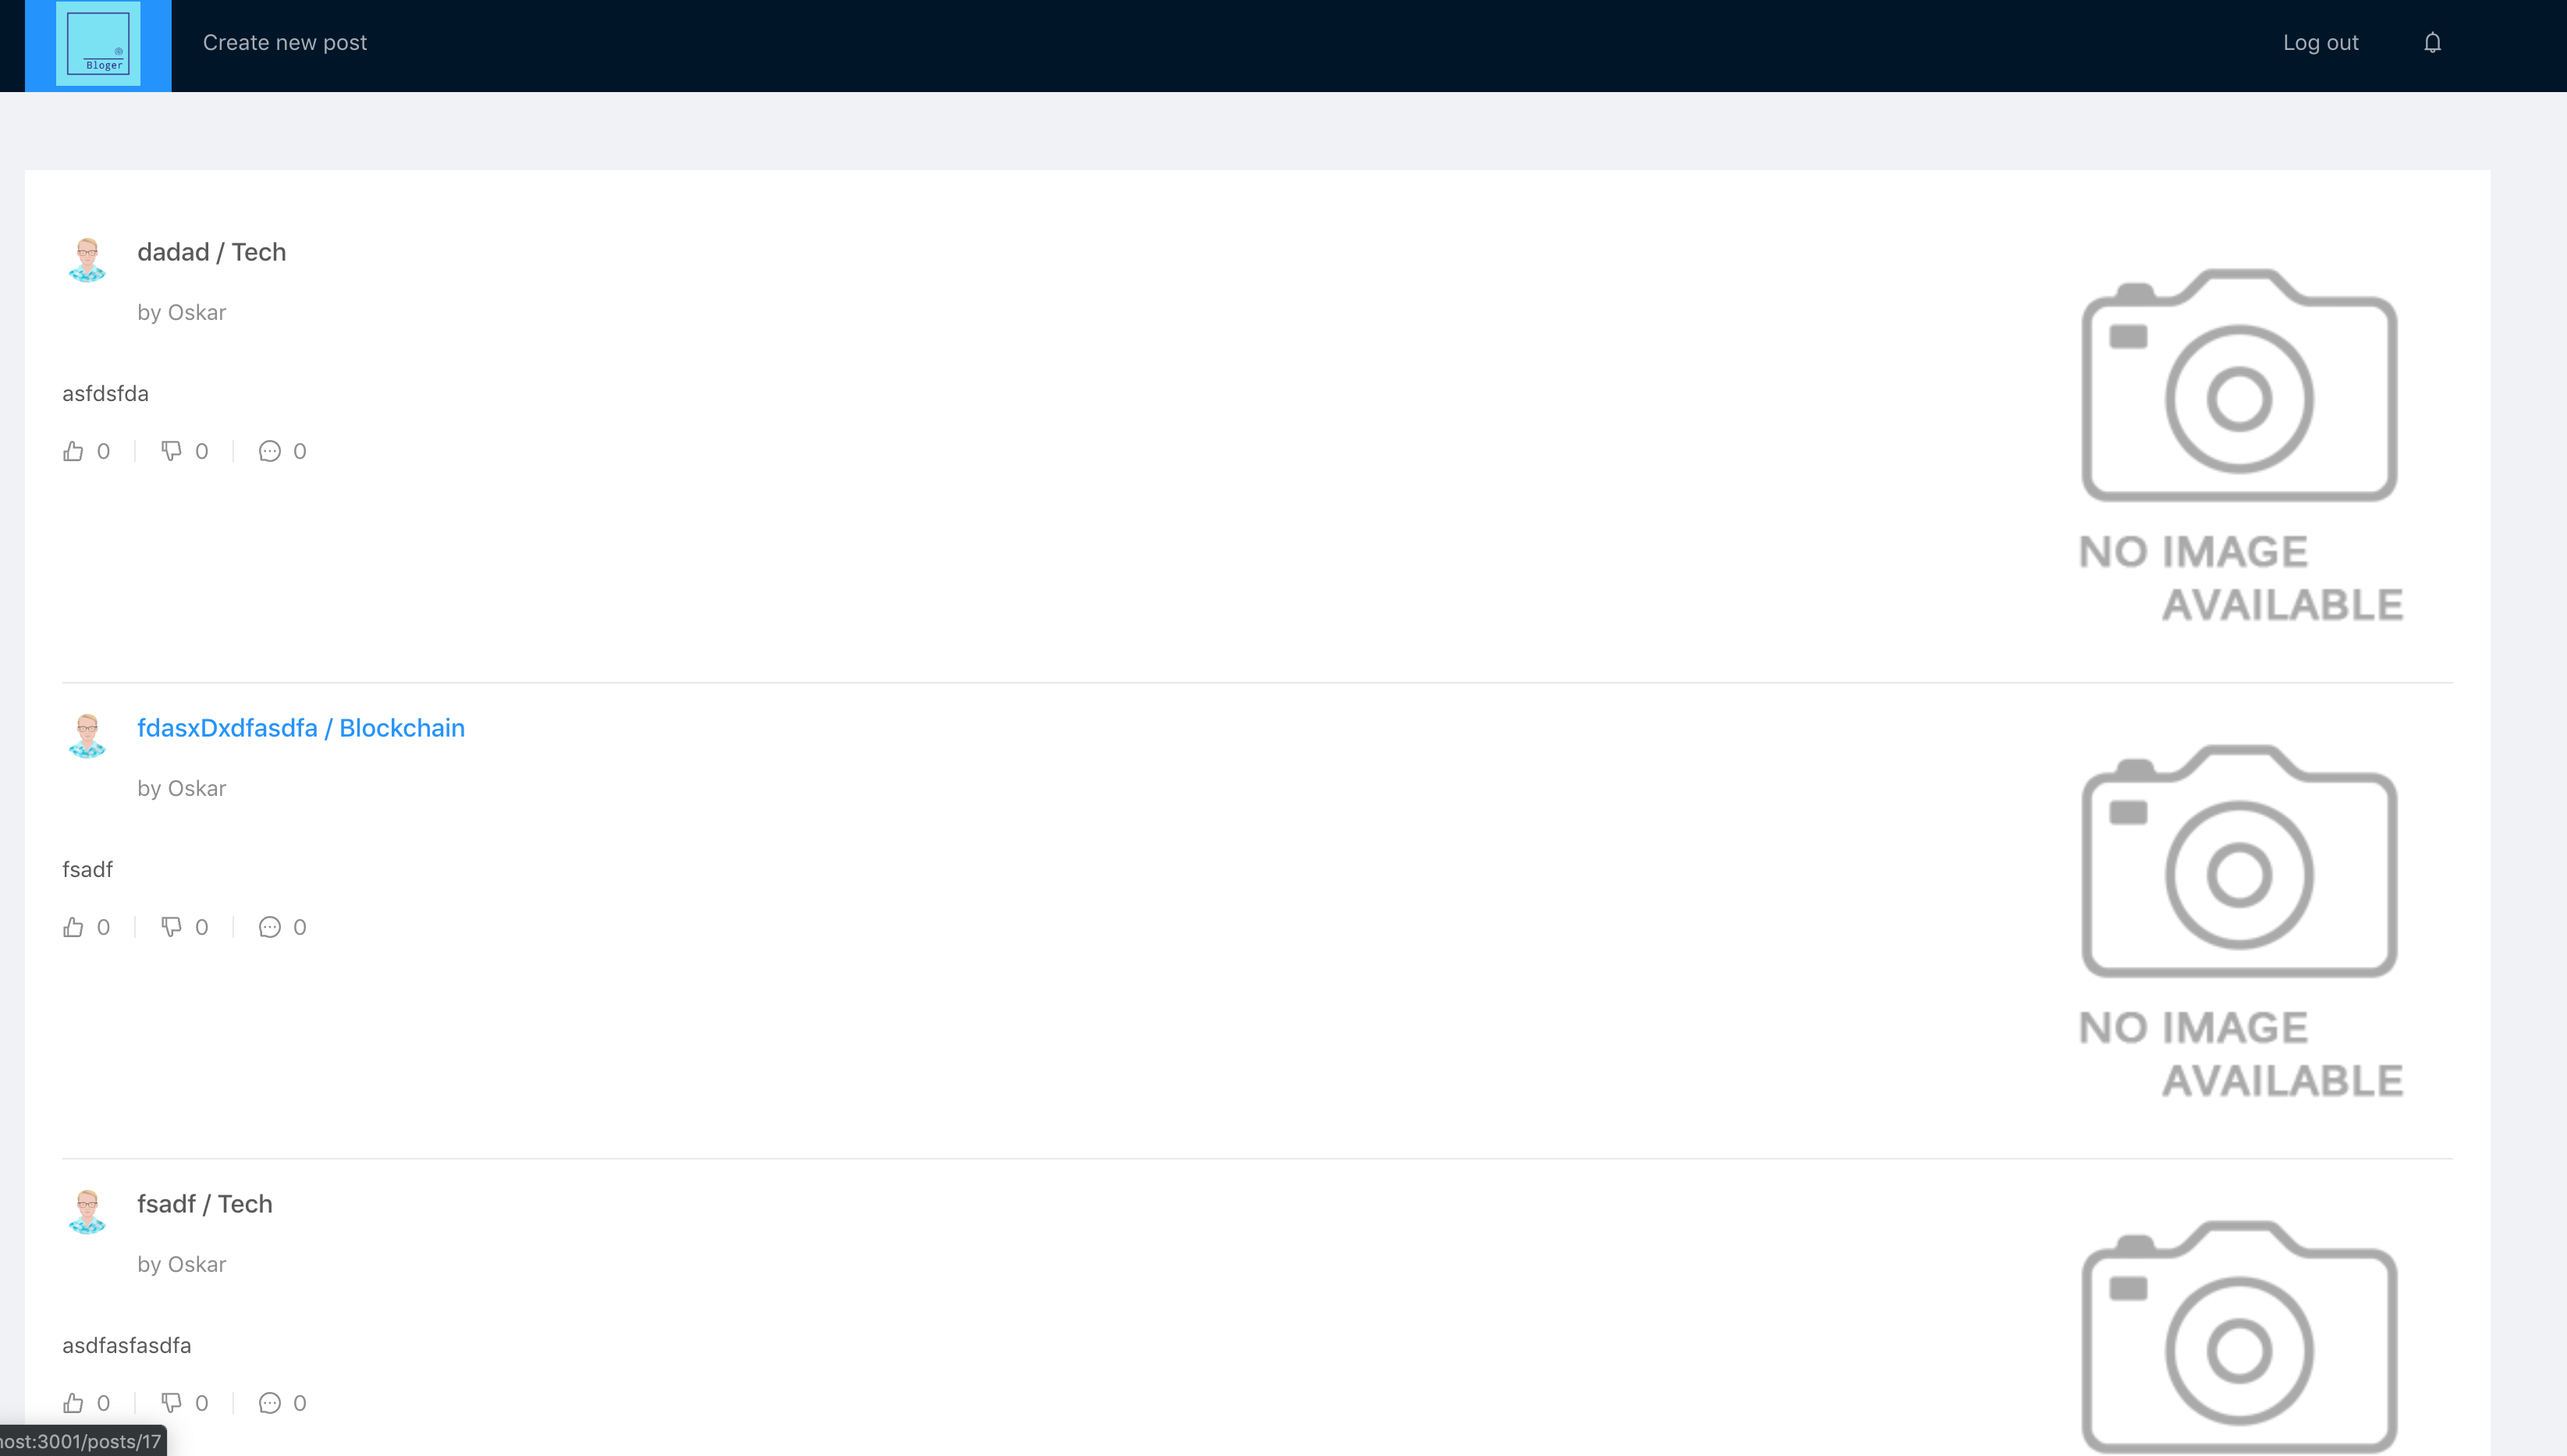
\includegraphics[width=\textwidth]{images/stronaglowna.png}
    \caption{Strona główna aplikacji}
    \label{fig:main_page}
\end{figure}[]

\subsubsection{Szczegółowy widok wpisu}
W tym widoku (rys. \ref{fig:post_view}) użytkownik ma dostęp do pełnej treści wpisu oraz komentarzy

\begin{figure}
    \centering
    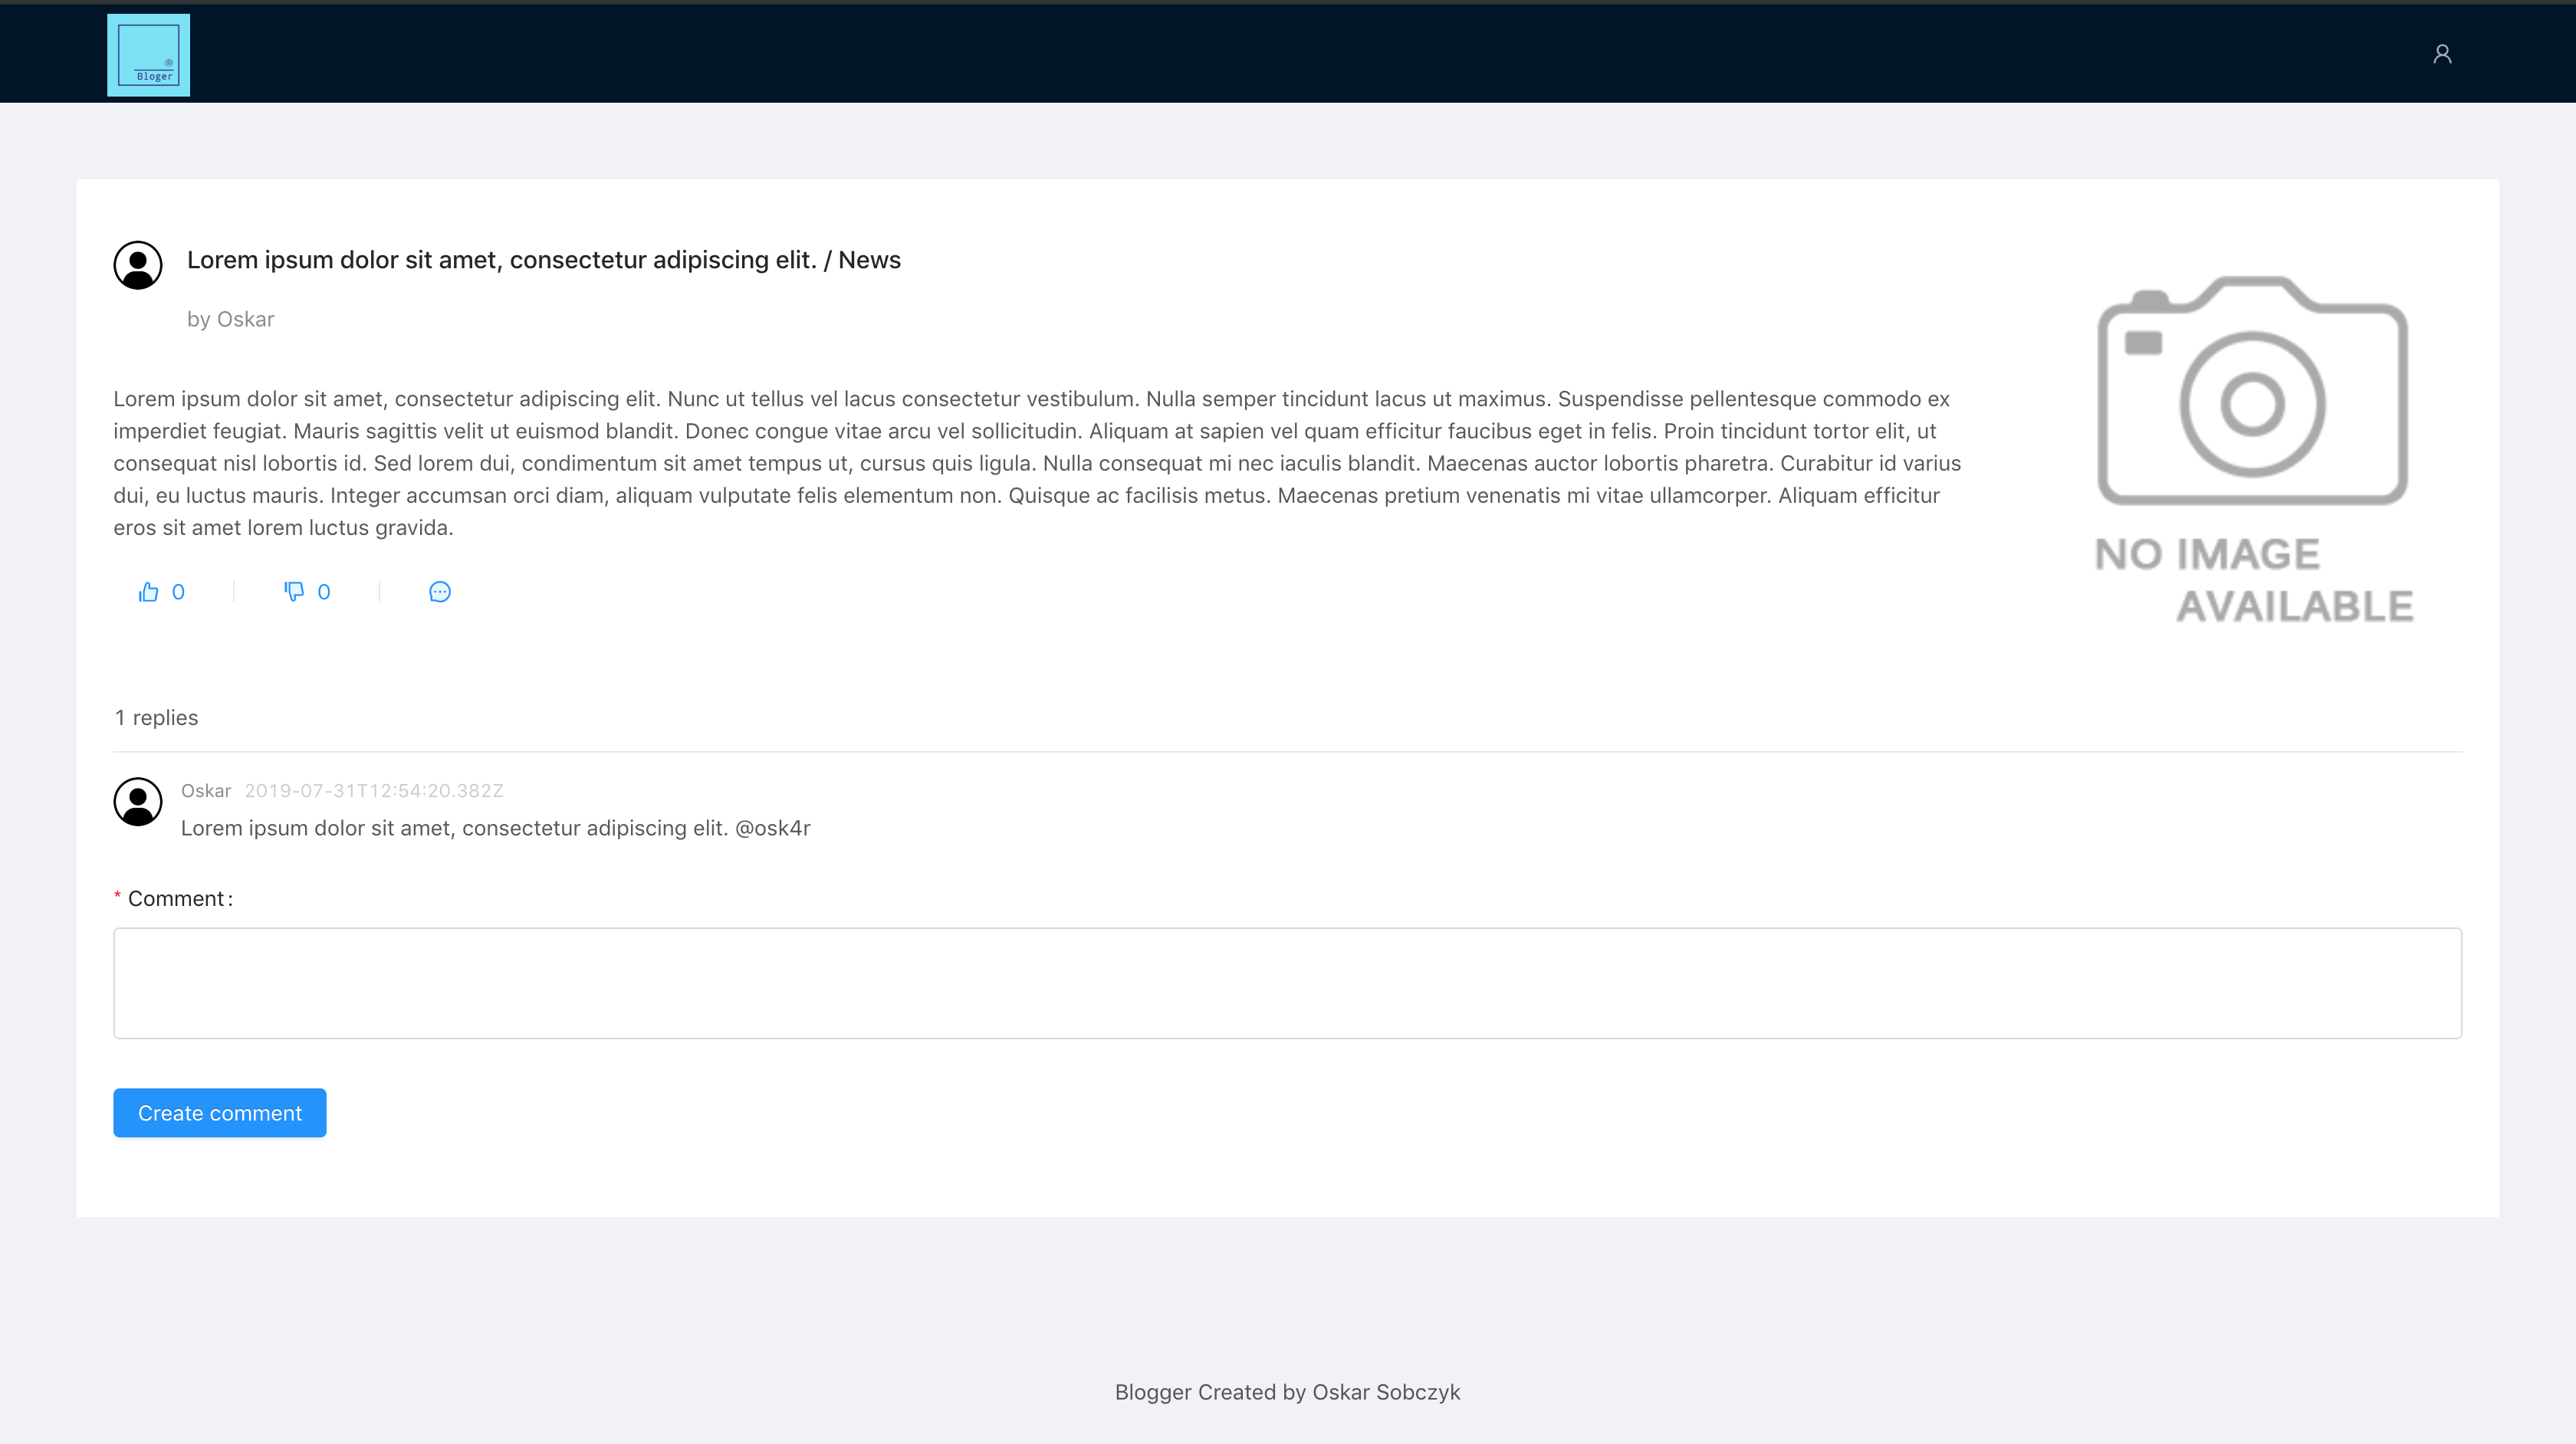
\includegraphics[width=\textwidth]{images/widok_postu.png}
    \caption{Widok szczegółowy}
    \label{fig:post_view}
\end{figure}

\subsubsection{Rejestracja nowego użytkownika}
Aby zarejestrować się w serwisie (rys. \ref{fig:register}), należ podać imię, nick, e-mail, hasło opcjonalnie użytkownik może dodać swój awatar. Po wysłaniu formularza, na podany wcześniej adres poczty zostanie wysłany link aktywujący konto.

\begin{figure}
    \centering
    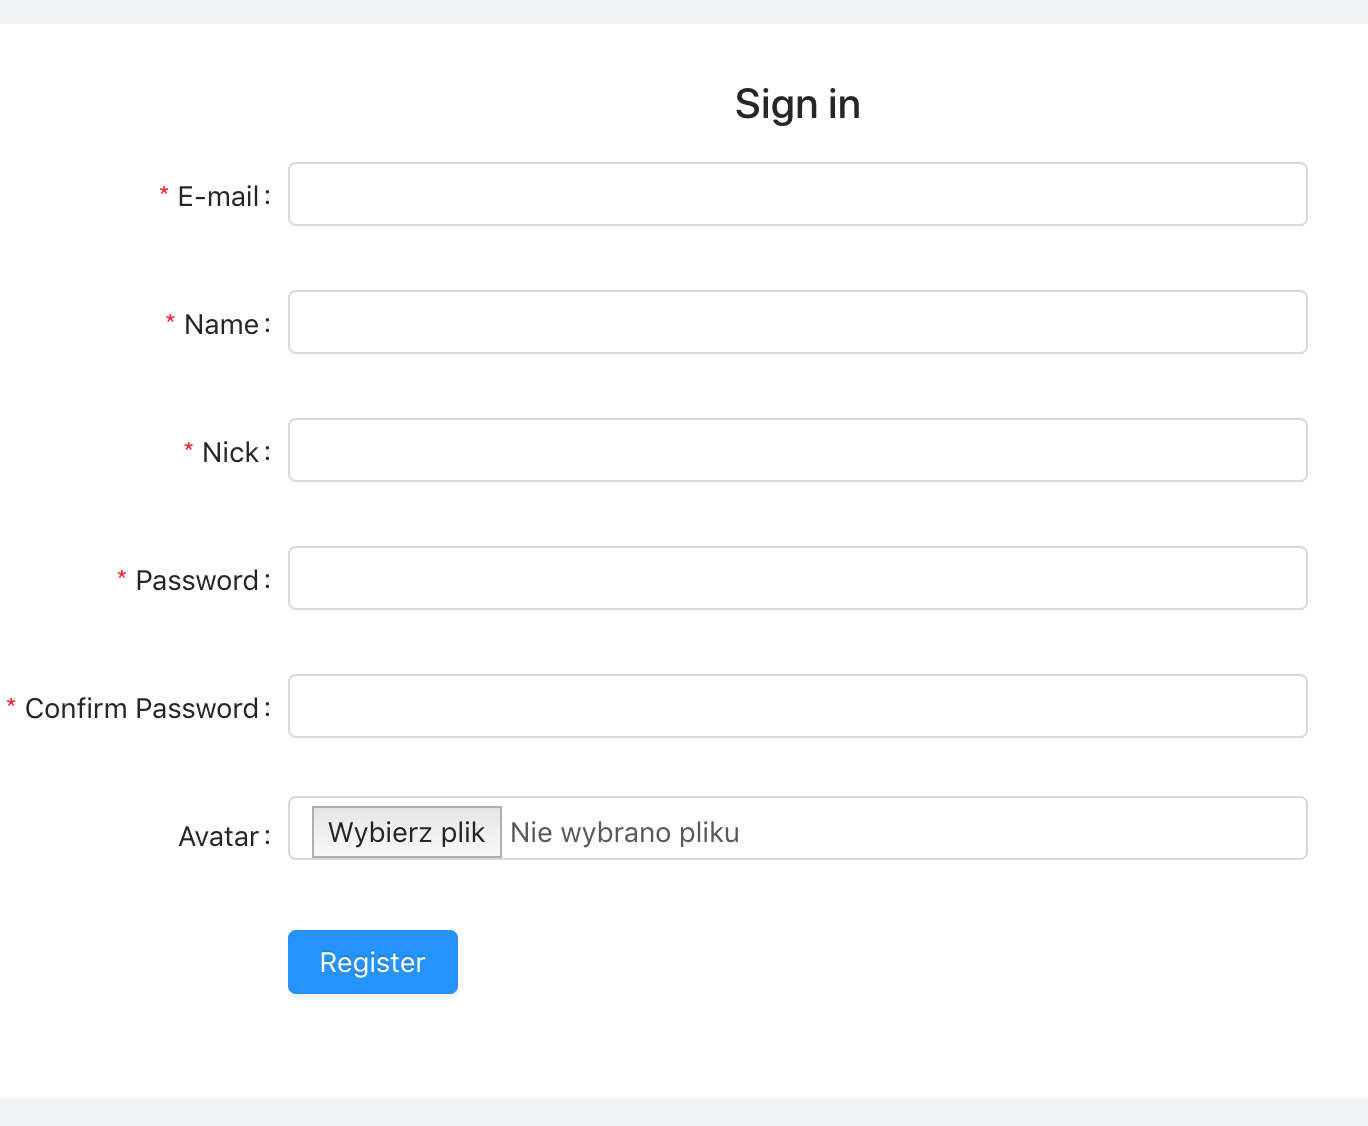
\includegraphics[width=\textwidth]{images/rejestracja.png}
    \caption{Formularz rejestracji nowego użytkownika}
    \label{fig:register}
\end{figure}

\subsubsection{Logowanie}
Aby móc korzystać ze wszystkich możliwości serwisu wymagane jest logowanie (rys. \ref{fig:login}). Możliwe jest tylko po wcześniejszej aktywacji konta. W tym celu należy podać adres e-mail oraz hasło.

\begin{figure}
    \centering
    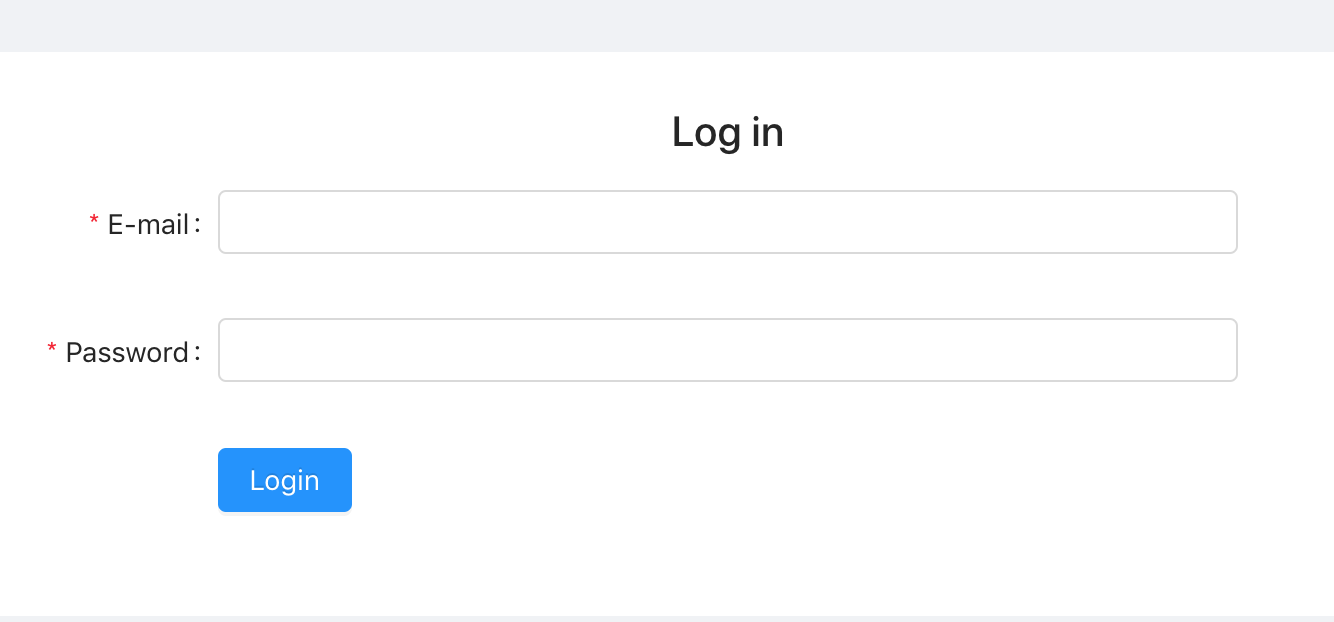
\includegraphics[width=\linewidth]{images/logowanie.png}
    \caption{Formularz logowania}
    \label{fig:login}
\end{figure}

\subsection{Zalogowany użytkownik}

\subsubsection{Dodawanie wpisów}
Zalogowany użytkownik może dodawać wpisy do serwisu. Aby tego dokonać, musi kliknąć przycisk znajdujący się w nagłówku strony \textit{,,Create new post"}, a następnie zostanie przekierowany do odpowiedniego formularza. Tam do wypełnienia będzie miał takie pola jak tytuł, treść, kategoria oraz miniaturka. Po wysłaniu oraz walidacji formularza wpis zostanie utworzony a użytkownik przeniesiony do niego.

\subsubsection{Ocenianie wpisów}
Każdy zalogowany użytkownik ma możliwość oceniania użytkowników. Wystarczy że klikniąć w łapkę w dół lub w górę przy danym poście (rys.\ref{fig:like}). 
\begin{figure}
    \centering
    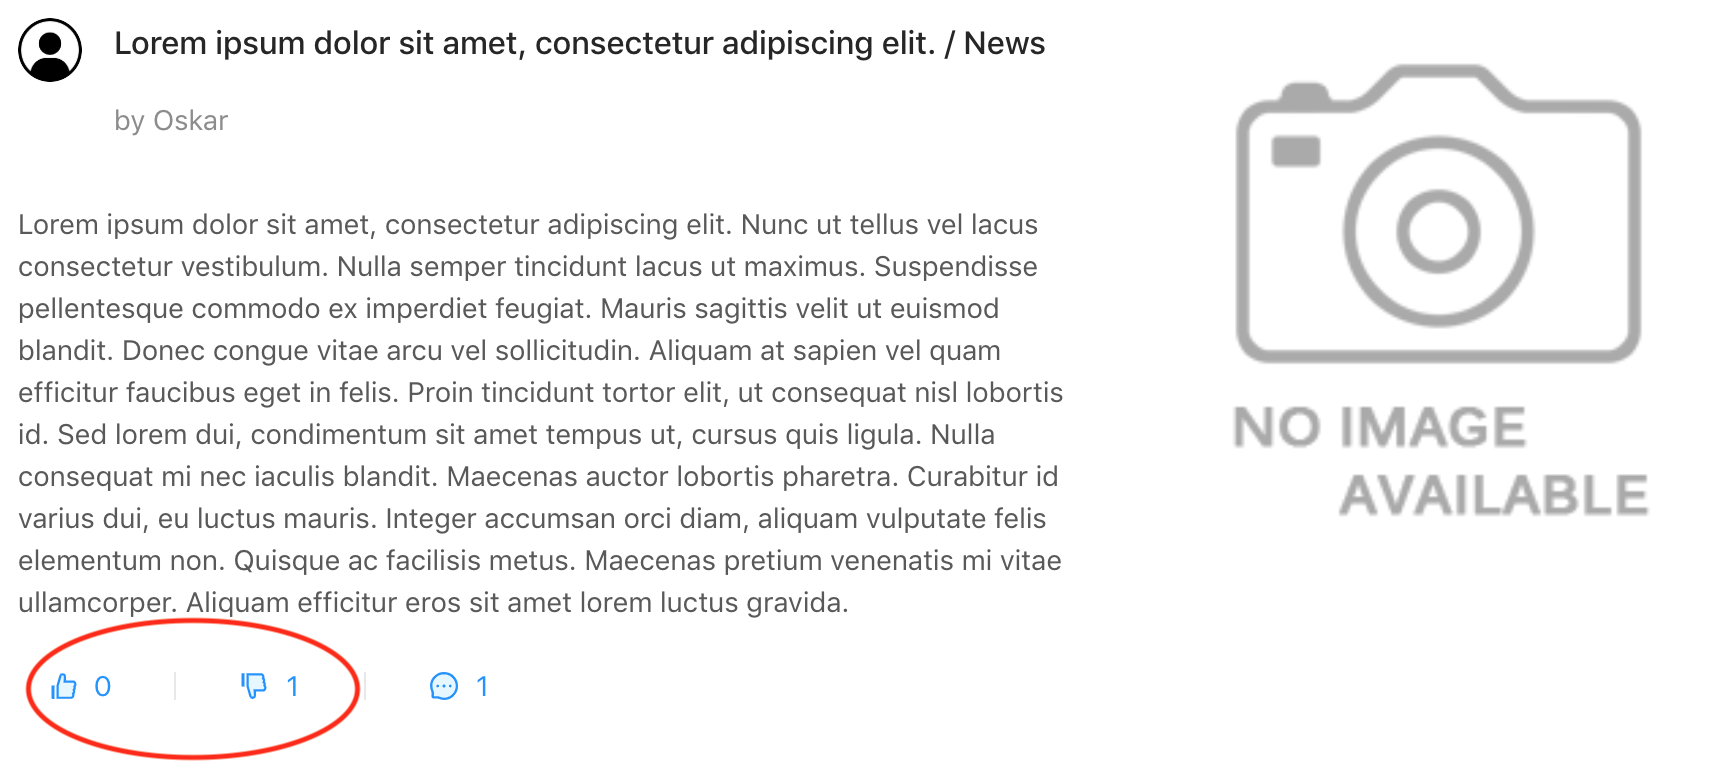
\includegraphics[width=\linewidth]{images/like.png}
    \caption{Ekran modułu oceniania}
    \label{fig:like}
\end{figure}

\subsubsection{Komentarze}
Dla zalogowanych użytkowników udostępniona została funkcja dyskusji na temat wpisów za pomocą komentarzy (rys. \ref{fig:comment}). Dodawanie nowych wpisów jest możliwe za pomocą formularza dostępnego w szczegółowym widoku wpisu. Dodatkowo w system komentarzy wbudowany jest system ,,wołania". Aby ,,zawołać" innego użytkownika w treści komentarza należy jego nick poprzedzić symbolem \textbf{\textit{,,@"}}. W ten sposób wspomniany użytkownik otrzyma powiadomienie o naszej aktywności (rys. \ref{fig:notification}).

\begin{figure}
    \centering
    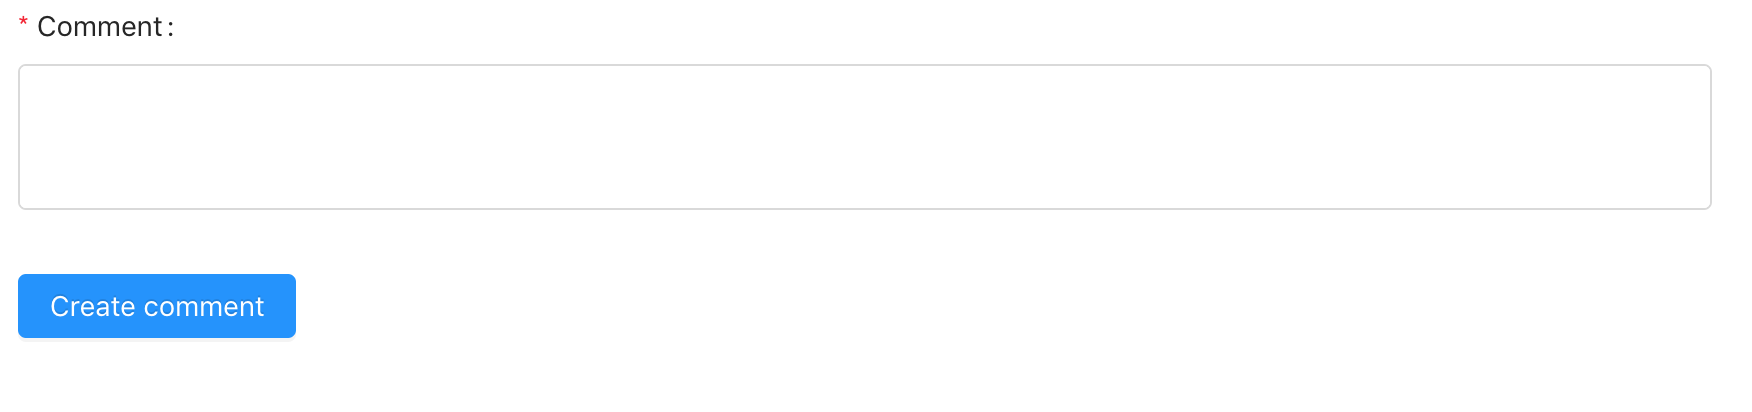
\includegraphics[width=\linewidth]{images/komentarz.png}
    \caption{Formularz komentarzy}
    \label{fig:comment}
\end{figure}

\subsection{Obszar powiadomień}
W tym miejscu (rys. \ref{fig:notification}) użytkownik ma dostęp do listy swoich powiadomień między innymi z komentarzy.
\begin{figure}
    \centering
    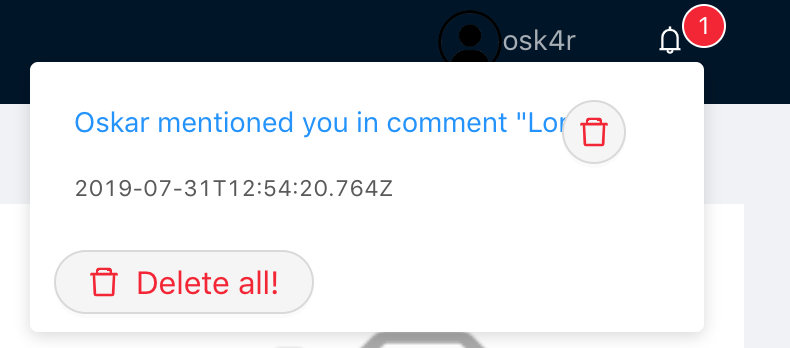
\includegraphics[width=\linewidth]{images/powiadomienia.png}
    \caption{Ekran obszaru powiadomień}
    \label{fig:notification}
\end{figure}

\section{Dostęp do działającego systemu}
Działający system jest dostępny pod adresem \ldots. Aby korzystać ze wszystkich możliwości serwisu, należy założyć konto i potwierdzić je klikając w otrzymany e-mailem link. Dostępne jest również konto testowe login: test hasło: test.

\chapter{Podsumowanie}
Celem pracy było utworzenie platformy blogowej łączącej funkcje serwisów Reddit oraz Medium. Do implementacji użyto nowoczesnych narzędzi takich jak frameworki React oraz Ruby on Rails. Pozwoliło to na stworzenie aplikacji spełniającej nowoczesne standardy programistyczne oraz z zakresu interfejsu użytkownika. Dzięki zastosowanym w systemie technologiom stanowi on solidną podstawę pozwalającą na dalszy rozwój. 

\section{Dalszy rozwój}

Biorąc pod uwagę skalę popularności serwisów o podobnej funkcjonalności, dalszy rozwój aplikacji może pozwolić na wypuszczenie jej na rynek komercyjny. Aby zwiększyć zaangażowanie użytkowników do serwisu, przydatny może być system powiadomień. Jego rozbudowa o nowe typy notyfikacji sprawi że odbiorcy częściej będą odwiedzać portal. W celu uatrakcyjnienia części wizualne przydatną funkcją będzie rozbudowa edytora wpisów o możliwość pogrubiania czcionki, kursywy czy zmiany jej wielkości. Należy wziąć pod uwagę że nie każdy użytkownik jest zainteresowany wszystkimi treściami. Umożliwienie personalizacji strony głównej przez możliwość wyboru z jakich kategorii mają być wyświetlane wiadomości. Dzięki zastosowanej architekturze oddzielającej aplikacje serwerową od interfejsu użytkownika, istnieje możliwość aby w przyszłości powstała aplikacja mobilna wykorzystująca React Native oraz już istniejące API.


%%%%% BIBLIOGRAFIA

%\begin{thebibliography}{1}
%\bibitem{example} \ldots
%\end{thebibliography}

\end{document}